\documentclass[11pt]{article}

% -----------------------------------------------------------------------------
% NEURO 120 Final Project
% Group 5: Georgia Hutchinson, JaKayla Harris, Djordje Ivanovic
% -----------------------------------------------------------------------------

\usepackage[margin=0.9in]{geometry}
\usepackage{titling}
\setlength{\droptitle}{-1.25em}
\usepackage{graphicx}
\usepackage{booktabs}
\usepackage{amsmath,amssymb}
\usepackage{caption}
\usepackage{subcaption}
\usepackage{microtype}
\usepackage{hyperref}
\usepackage{xurl}
\hypersetup{colorlinks=true, linkcolor=black, urlcolor=blue, citecolor=black}
\usepackage[numbers,sort&compress]{natbib}
\usepackage{placeins}
\setlength{\parskip}{2pt}
\linespread{1.1}

\graphicspath{{results/figures/}}
\captionsetup{font=small,labelfont=bf}
\newcommand{\divg}{\mathcal{D}}

\title{%
  \textbf{Do song-selective electrodes carry more song-vs-music information?}\protect\\[0.35em]
  {\large\textbf{A re-analysis of Norman--Haignere et al.\ (2022) with a Bellier et al.\ (2023) extension}}%
}
\author{%
  Georgia Hutchinson \quad JaKayla Harris \quad Djordje Ivanovic\\[0.35em]
  {\small Group 5 \;\textbar\; NEURO 120 (Spring 2026)}\\[0.55em]
  {\footnotesize\textbf{Code:}\quad\protect\url{https://github.com/djordjeivanovic11/neuro120-project}}%
}
\date{\today}

\begin{document}
\maketitle
\vspace{-1.75em}
% =============================================================================
\begin{abstract}
\noindent\textbf{Question.}\quad
Do the brain regions that respond most strongly to song also carry the most \emph{information} a decoder could use to separate song from instrumental music?

\smallskip
\noindent\textbf{Replicate vs.\ original.}\quad
We replicate decoding and representational geometry on the published \citet{NormanHaignere2022} song/speech/music subset (33 electrocorticography, ECoG, electrodes; 49 stimuli; 0--2~s trial windows). Our original contributions are (i) a matched 7-vs-7 random-subset null that controls for subset-size confounds, (ii) ridge acoustic partialling on residuals to test for structure not linearly predicted by a cochleogram + spectrotemporal-modulation feature bank, and (iii) a \citet{Bellier2023} continuous-music extension using a vocal-vs-instrumental decoder with interleaved blocked-time cross-validation.

\smallskip
\noindent\textbf{Findings.}\quad
Under the fair 7-vs-7 null, the seven song-selective electrodes are not privileged: balanced accuracy sits slightly below the random-draw mean (one-sided $p = 0.63$) and representational dissimilarity matrix (RDM) divergence modestly above it ($p = 0.35$); neither lies in the upper tail. Linearly subtracting low-level acoustics removes most of the divergence but leaves a residual ($0.33/0.39/0.47$ of the raw peak across song-only / all / no-song subsets), borderline-significant only for song-only ($p = 0.052$). On Bellier, the vocal-vs-instrumental decoder reaches $\approx 0.78$ balanced accuracy on the full 2395-electrode supergrid, with right-STG $>$ left-STG in the same direction as the published report.

\smallskip
\noindent\textbf{Bottom line.}\quad
Song-selective electrodes are informative but not privileged under a size-matched information test, and the song-vs-music signal is largely, though not entirely, predictable from low-level acoustics.
\end{abstract}

% =============================================================================
\section{Introduction}\label{sec:intro}
% =============================================================================

People separate speech, song, and instrumental music almost effortlessly. Listeners can tell voice from non-voice sounds within tens of milliseconds \citep{Mesgarani2014}, and fMRI voxel-decomposition work has shown that music and speech sit on largely distinct cortical pathways in human auditory cortex \citep{NormanHaignere2015}. Less is known about how the brain differentiates instrumental music from vocal music (song), which combines those two pathways.

\citet{NormanHaignere2022} took the first direct electrophysiology step toward an answer. They recorded ECoG responses to 165 natural sounds and decomposed the electrode responses into hypothesis-free components. One component responded more strongly to song than to either speech or instrumental music, and this song response could not be rewritten as a combination of the speech- and music-selective components. Seven ECoG electrodes were flagged as ``song-selective.'' These seven electrodes are the starting point for our project.

\paragraph{What we ask.} The \citet{NormanHaignere2022} labels are defined on the \emph{average} response magnitude: a song-selective electrode is one whose mean response is higher to song than to other sounds. But firing strongly and carrying useful information are not the same thing. Imagine a light that flashes brightly whenever there is sound of any kind: it responds strongly, but it does not help you tell song apart from music. An electrode that always fires more during song might in principle do the same thing. So we asked what happens when we probe these electrodes with a decoder instead. Specifically:

\begin{enumerate}
\setlength{\itemsep}{0pt}
    \item \textbf{Are song-selective electrodes actually better at separating song from instrumental music than other auditory-cortex electrodes?}
    \item \textbf{When does the song-vs-instrumental difference appear over time, and does it stay stable?}
    \item \textbf{Is the difference mostly explained by low-level acoustics, or does some of it remain after acoustics are controlled for?}
\end{enumerate}

Question (1) is the central one, and it has a built-in pitfall. Smaller electrode sets are easier for a linear decoder to fit, so comparing 7 song electrodes directly against all 33 electrodes would confound subset size with selectivity. To avoid this, we built a fair comparison group. We drew 7 electrodes at random from the pool of \emph{non}-song electrodes, measured how well those 7 decode song from music, and repeated this 1000 times. We call each such draw a \emph{matched random subset}: same size as the song-selective group (7), but from electrodes that are \emph{not} labelled song-selective. If the song electrodes are truly special, their decoder score should sit in the upper tail of this distribution. If not, random size-matched non-song subsets will often score as well as or better than the song-selective set under the same pipeline---which is what we observe for balanced accuracy, while RDM divergence sits only modestly above the random-draw mean without reaching the upper tail.

Question (3) is motivated by what is already known about the superior temporal gyrus (STG), the cortical region most electrodes in both datasets sit on. A large fraction of STG responses to complex sounds is explained by cochleogram and spectrotemporal-modulation statistics \citep{Mesgarani2014,Hullett2016,Hamilton2018}, but phonetic, prosodic, and melodic structure also contribute \citep{Yi2019,Sankaran2024,Leonard2024}. If the song-vs-music signal turns out to be a pure re-encoding of acoustics, there is nothing song-specific left to explain. If part of it survives after acoustics are controlled for, auditory cortex may still carry song-vs-music structure that is not linearly predicted by that specific acoustic feature bank.

\paragraph{Does it hold in continuous music?} Short, repeated stimuli are convenient for trial-averaging but may not generalise to natural listening \citep{HamiltonHuth2020}. We therefore re-run question (1) on the \citet{Bellier2023} dataset: ECoG from 29 patients listening to a continuous 191-second excerpt of Pink Floyd's \emph{Another Brick in the Wall, Part 1}, with hundreds of electrodes per patient. This extension is deliberately bounded: one decoder, one anatomical split, one temporal-profile comparison. The goal is to check whether our central finding survives a very different stimulus regime, not to build a second project around the dataset.

% =============================================================================
\section{Methods}\label{sec:methods}
% =============================================================================

\subsection{Data}
We used two publicly available human electrocorticography (ECoG) datasets. ECoG records electrical activity directly from electrodes placed on the cortical surface of neurosurgical patients, which provides high temporal resolution and good spatial coverage of auditory cortex. Both datasets provide preprocessed high-frequency brain activity (HFA), the standard ECoG proxy for local cortical firing rate.

\paragraph{Norman--Haignere (2022).} Our main dataset is per-electrode HFA in 15 patients in response to 165 natural sounds, trial-averaged and sampled at 75 points across a 2-second trial window. We kept the three coarse classes relevant to our question: \textsf{song} ($n = 11$), \textsf{speech} (English + foreign, $n = 17$), and \textsf{music} (instrumental, $n = 21$). This left 49 stimuli and 33 electrodes. Each electrode comes with a selectivity label (song, speech, or music) from \citet{NormanHaignere2022}, defined on the full 165-stimulus task using trial-averaged response magnitudes.

\paragraph{Bellier (2023).} Our second dataset is a 29-patient ECoG recording of people listening to a 190.72-second excerpt of a Pink Floyd song, sampled at 100~Hz. For each patient we dropped channels flagged as reference, noisy, or epileptic and attached FreeSurfer anatomical labels from the companion file. Concatenating patients along the electrode axis gives a cross-patient matrix of shape $(T, N) = (19072, 2395)$. We call this the \emph{supergrid}: a single stacked matrix with 19072 time samples across 2395 electrodes pooled across all 29 patients, which is the object every downstream Bellier analysis runs on. We derive a binary \texttt{vocal\_present} mask for the stimulus from hand-segmented vocal intervals (annotation procedure in \S\ref{sec:methods:bellier}); for our coarse vocal-vs-instrumental decoder, time samples outside those intervals are treated as non-vocal.

\paragraph{Acoustic features.} To later ask how much of the neural signal is just low-level audio, we loaded two feature matrices released with Norman--Haignere: a cochleogram $F_{\mathrm{coch}} \in \mathbb{R}^{165 \times 6}$ (spectral energy in six frequency bands) and a spectrotemporal-modulation tensor $F_{\mathrm{mod}} \in \mathbb{R}^{165 \times 7 \times 9}$ (how energy moves across frequency and time). We flattened $F_{\mathrm{mod}}$ to $165 \times 63$ and orthogonalised it column-wise against $F_{\mathrm{coch}}$ by ordinary least squares (OLS) regression, following the reference MATLAB code of \citet{NormanHaignere2022}; this prevents the two feature blocks from double-counting overlapping variance. After aligning to our 49-stimulus subset, the acoustic regressor matrix is $A = [F_{\mathrm{coch}} \mid F_{\mathrm{mod,resid}}] \in \mathbb{R}^{49 \times 69}$.

\subsection{Analytical approach}
We addressed question~(1) with a linear song-vs-music decoder and a classifier-free RDM divergence score, each evaluated under the same matched 7-vs-7 random-subset control. Question~(2) was addressed with time-resolved decoding and divergence, cross-temporal train--test matrices, and (for Bellier) a time-blocked binary decoder on sliding windows. Question~(3) used ridge acoustic partialling at every time window, recomputing divergence on the residual. Complementary analyses were leave-one-electrode-out importance, non-linear decoder controls on Norman, and shape-matched HFA profiles across Norman and Bellier.

\begin{table}[t]
\centering
{\footnotesize
\noindent\resizebox{\textwidth}{!}{%
\begin{tabular}{p{0.28\linewidth} p{0.34\linewidth} p{0.34\linewidth}}
\toprule
Research question & Analysis & What it tests \\
\midrule
Are song-selective electrodes privileged? & Song-vs-music decoder and RDM divergence under a matched 7-vs-7 random-subset null & Whether the seven song electrodes outperform size-matched non-song groups \\
When does the signal appear, and is it stable? & Time-resolved decoding and divergence; cross-temporal train--test matrices; Bellier sliding-window decoder & Timing and stability of song-vs-music information (Norman trial; Bellier continuous) \\
Is the signal mostly acoustic? & Ridge acoustic partialling; RDM divergence on residuals & Whether geometry remains after linear removal of low-level acoustic features \\
Does the result generalise to natural listening? & Bellier vocal-vs-instrumental decoder; cross-dataset temporal profiles & Distributed vocal/instrumental signal in continuous music \\
\bottomrule
\end{tabular}}}
\caption{Roadmap linking research questions to analyses.}
\label{tab:methods-roadmap}
\end{table}

\subsection{Decoding}
Our first measure of song-vs-music information is a supervised decoder: given a neural feature vector, how well can a simple classifier predict the stimulus class? A high score means the information is there in a form a downstream brain region could use.

We reduce each trial to a feature vector by averaging the HFA inside a short time window, producing one value per electrode. For the ``early-window'' analyses we use a single $[0.2, 0.6]$~s window. This bracket starts roughly one HFA sample after stimulus onset (past the onset transient) and ends around the peak of the classic STG category responses \citep{NormanHaignere2022,Hamilton2018}, so it covers the post-onset epoch where category information is concentrated. For time-resolved analyses we use sliding windows of width $0.15$~s and step $0.05$~s. A $0.15$~s window spans about 11 of the 75 time samples in the trial (a non-trivial local average but still short compared with the trial), and the $0.05$~s step gives $\approx 40$ overlapping windows, dense enough to draw a smooth time course.

All decoding uses $L_2$-penalised logistic regression with per-fold standardisation ($C = 1$), the standard choice for cognitive ECoG \citep{Holdgraf2017}. We report \emph{balanced accuracy} (bacc), the unweighted average of per-class recall (each class counts equally).\footnote{Balanced accuracy is the mean of ``fraction correct within class~1,'' ``fraction correct within class~2,'' and so on. Plain accuracy is dominated by whichever class has more trials, so a classifier that always guesses the majority class can look good without carrying real class information. We use bacc throughout for unequal class sizes.} Cross-validation (CV) uses stratified group 5-fold splits with stimulus ID as the grouping variable, repeated 20 times with different random seeds for the headline numbers. Grouping by stimulus is essential: without it, the classifier could cheat by memorising a stimulus it saw during training, inflating accuracy without reflecting class-level information.

\subsection{Divergence: a classifier-free separation score}\label{sec:methods:divergence}
Decoding asks whether a classifier \emph{can} separate the classes. We also wanted a geometric measure, independent of any classifier, that asks how structured the neural responses are in the first place. For this we use a representational dissimilarity matrix (RDM): in one sentence, a square table of how ``far apart'' every pair of stimuli is in neural response space, so we can ask whether song trials and music trials form separable clusters without fitting a classifier. If category is reflected in neural geometry, pairs of stimuli from different classes should sit farther apart in the RDM than pairs from the same class.

Let $M \in \mathbb{R}^{N_s \times N_e}$ be the window-averaged feature matrix (one row per stimulus, one column per electrode). We $z$-score each column so no single electrode dominates the distance, and define the RDM $R$ by correlation distance between stimulus rows, $R_{ij} = 1 - \mathrm{corr}(z(M_i), z(M_j))$. Correlation distance compares response \emph{patterns} rather than absolute magnitudes, which is a standard choice in representational similarity analysis (RSA). For a pair of classes $(a, b)$ the \emph{divergence} is the mean between-class pairwise distance minus the average within-class distance:
\begin{equation}
  \divg(a, b) \;=\; \underbrace{\overline{R_{ab}}}_{\text{between}} \;-\; \tfrac{1}{2}\!\left(\underbrace{\overline{R_{aa}}}_{\text{within-}a} + \underbrace{\overline{R_{bb}}}_{\text{within-}b}\right),
\label{eq:divergence}
\end{equation}
where $\overline{R_{ab}}$ is the mean of the off-diagonal block between labels $a$ and $b$, and $\overline{R_{aa}}$ is the mean of the strictly upper-triangular entries inside the class-$a$ block. In plain words: we compare \emph{how different are song responses from music responses} against \emph{how different are songs from other songs, and music from other music}. A positive divergence means cross-class stimuli are farther apart than same-class stimuli, so the classes are genuinely separated in neural space. We use this score rather than, say, decoder margin because it does not need a classifier, and because its numerator and denominator live on the same distance scale, so changes in the number map cleanly onto geometric changes in the RDM.

\subsection{Significance testing}
Every headline number is backed by one or more of three controls. Each asks a different question about where the effect could have come from by chance.
\begin{enumerate}
\setlength{\itemsep}{1pt}
    \item \textbf{Bootstrap over stimuli.} We resample stimulus IDs within-class with replacement, deduplicate to avoid zero-distance self-pairs, recompute the divergence curve, and report a percentile 95\% confidence interval (CI) across $B=1000$ resamples. This tells us how reliable the number is across resamples of the stimuli.
    \item \textbf{Label-shuffle permutation.} To build a chance baseline, we randomly reassign the class labels among the stimuli (within the $\{a,b\}$ pair only) and recompute the divergence 1000 times. At each time window we record the 95th percentile of these shuffled divergences, which we call the \emph{chance-level band}. Any curve sitting below this band is indistinguishable from what you would get with random labels. The peak $p$-value is $(\#\{\text{null peak} \geq \text{obs peak}\}+1)/(n_\text{perm}+1)$.
    \item \textbf{Matched random-subset control.} The song-selective set has only 7 electrodes, so we cannot compare it directly against all 33 electrodes without confounding group size with selectivity. Instead, we build a fair baseline by drawing 7 electrodes at random (without replacement) from the non-song pool, recomputing bacc and divergence, and repeating 1000 times. We then compare the observed song-only value to this distribution. If song-selective electrodes carry privileged information, the song-only score should sit in the upper tail; if not, it sits somewhere in the middle.
\end{enumerate}

\subsection{Controlling for low-level acoustics}\label{sec:methods:acoustic}
Songs and instrumental music sound different at the most basic level: songs have voices, different pitch patterns, different rhythms. So any brain region that separates song from music might just be picking up on those basic sound differences, not anything deeply ``musical.'' To test this we use a technique called linear partialling: we predict the neural signal from a bank of basic sound features, subtract out that prediction, and ask whether song-vs-music geometry remains in the residual. Anything left is, by construction, not explainable by a linear readout of those features.

Concretely, at every sliding window we fit a ridge regression from the acoustic features $A$ to the neural matrix $M$, then replace $M$ by the residual: what the neural signal looks like \emph{after} subtracting out the predicted acoustic contribution. With centred columns $\tilde{A} = A - \bar{A}$ and $\tilde{M}_0 = M - \bar{M}$, the ridge coefficients $\hat{\beta}$ and the residual $\tilde{M}$ are
\begin{equation}
  \hat{\beta} \;=\; \left(\tilde{A}^{\!\top}\tilde{A} + \lambda I\right)^{-1}\tilde{A}^{\!\top}\tilde{M}_0,
  \qquad
  \tilde{M} \;=\; \tilde{M}_0 \;-\; \tilde{A}\,\hat{\beta}.
\end{equation}
The ridge penalty $\lambda$ is there for numerical stability: $A$ has 69 columns and only 49 rows, which makes the uncorrected inverse ill-conditioned. Very small $\lambda$ lets the regression chase noise; very large $\lambda$ under-removes real acoustic structure and biases the partialled divergence upwards. We use $\lambda = 1$ as a moderate compromise and confirmed on a small sweep that the qualitative pattern (surviving fraction $\approx 1/3$, similar ordering across subsets) is stable for $\lambda \in [0.1, 10]$. The RDM and divergence are then recomputed from $\tilde{M}$. For the permutation test we re-fit the regression inside every shuffle rather than fitting once. This ensures the null reflects neural geometry \emph{after} acoustics are controlled for, rather than inheriting a shortcut whenever the acoustic features themselves carry class information.

\subsection{Cross-temporal generalisation}
So far we have asked when during the trial the song-vs-music distinction is strongest. \emph{Cross-temporal generalisation} means: train the decoder at one time in the trial and test it at another---if performance stays high away from the diagonal of the resulting $N_t\times N_t$ train--test matrix, the underlying pattern is stable across time rather than locked to a single transient moment. A deeper question is whether the brain uses the \emph{same} neural code the whole time, or whether the pattern shifts as the sound plays. A stable code throughout the trial is the signature of a sustained categorical representation; a drifting code is the signature of an onset-driven one. We test this by training a classifier at one time and testing it at another: if a classifier trained at $t_i$ still works at $t_j$, the code is stable across that interval; if it fails, the code at $t_i$ is a different representation from the one at $t_j$. We train $L_2$ logistic regression on the song-vs-music task at each source window $t_i$, then test it at every destination window $t_j$ on held-out stimuli from the same CV split. Stacking all $(t_i, t_j)$ pairs gives an $N_t \times N_t$ bacc matrix: bright off-diagonals mean a stable code, dark off-diagonals mean it drifts. For a compact summary we compare the mean of the diagonal ($t_i = t_j$) against the mean of off-diagonal entries with $|t_i - t_j| \geq 0.25$~s. We use $0.25$~s as a conservative buffer (several sliding-window widths) so the off-diagonal mean does not inherit same-window overlap.

\subsection{Leave-one-out}
The random-subset control tests song electrodes as a group. A complementary question is whether any individual electrode contributes disproportionately, and whether those contributions concentrate in the song group. For each electrode $i$ we compute how much performance drops when it is removed: $\Delta_i = \text{bacc}(\text{all}) - \text{bacc}(\text{all} \setminus \{i\})$, and $\Delta_i^{\divg}$ the same way for divergence. To test whether song electrodes contribute more than others on average, we run a group-label permutation test with 1000 shuffles, comparing the mean $\Delta$ inside the song group against the mean outside. We prefer a permutation test over a $t$-test here because the per-electrode $\Delta$ values are small, non-normal, and have unequal variance across groups.

\subsection{Bellier extension: vocal-vs-instrumental decoding}\label{sec:methods:bellier}
To check whether the central finding generalises beyond short repeated clips, we re-ran a simpler version of our decoder on Bellier. Instead of three coarse classes, we tested the binary question the stimulus allows: can we decode when there is vocal content versus when there is not? This also lets us test the anatomical claim of \citet{Bellier2023} that the vocal signal is stronger in right STG than left STG.

We tiled the supergrid with $500$~ms windows at $100$~ms step (1903 windows in total) and labelled each window \texttt{vocal} if more than 50\% of its samples fell inside a manually annotated vocal interval. A $500$~ms window is long enough to span a sung syllable or two (the natural unit of the vocal/instrumental contrast in continuous song) while still being short compared with the 191-second song. The $100$~ms step gives dense temporal coverage without creating near-duplicate windows. The 50\% threshold is a simple majority rule: a window straddling a vocal/instrumental boundary is assigned to whichever class dominates it.

\paragraph{Vocal annotation and limitations.}
The vocal intervals were manually annotated by the project team by listening to the stimulus audio and marking periods in which lead vocal content was clearly present. We used a coarse binary rule rather than phoneme- or syllable-level alignment because the Bellier extension is a naturalistic vocal-vs-instrumental check, not a fine-grained speech-alignment study. We did not collect a second rater or compute inter-rater reliability, so exact boundary placement is a limitation. The majority-overlap window rule above reduces sensitivity to small boundary shifts by assigning borderline windows to whichever label occupies most of the 500~ms tile.

We analysed four electrode subsets: \textsf{all} (the full 2395-electrode supergrid), \textsf{right\_STG}, \textsf{left\_STG}, and \textsf{non\_STG}. The STG subsets use FreeSurfer \texttt{superiortemporal} labels split by the \texttt{ctx-lh} / \texttt{ctx-rh} prefix.

\paragraph{Blocked-time CV with interleaved folds.} Continuous-stimulus ECoG needs a time-blocked CV scheme because adjacent samples are correlated, so random splits would leak information between train and test. A contiguous 5-fold split is the obvious first try, but it breaks here: the vocal annotations cover only the first $\approx 92$~s of the 191~s song, so folds 3 and 4 of a contiguous split fall entirely in the instrumental region and balanced accuracy is undefined on them. We fix this with \emph{interleaved blocked folds}. The intuition is like dealing cards: we chop the song into 15 shorter contiguous blocks and deal them into 5 folds, so each fold is the union of three non-adjacent segments that are spread across the recording. Formally, we divide time into $n_\text{folds} \times n_\text{blocks/fold} = 15$ equal contiguous blocks and assign block $b$ to fold $b \bmod n_\text{folds}$. Every fold then contains both vocal and instrumental windows, no single 500~ms window crosses a fold boundary, and within-segment autocorrelation is preserved.

On these folds we fit $L_2$ logistic regression with \texttt{LogisticRegressionCV} ($C \in \{10^{-3}, \dots, 10^{3}\}$, inner 3-fold) on the electrode-means of each window. We report both balanced accuracy and the area under the ROC curve (ROC-AUC), the latter being a threshold-free summary of how well the decoder's continuous scores separate the two classes. We only run a more expensive non-linear model on subsets that already show a clear linear signal, so our small convolutional neural network (CNN; \texttt{TinyTemporalCNN}: two 1-D convolutions, adaptive pooling, linear head, 40 training epochs) is restricted to subsets whose logistic regression clears chance by at least $0.05$ bacc. Logistic regression always uses every contact in the named subset; when that count exceeds 256 electrodes, the CNN sees a deterministic subsample of 256 channels so the first convolution stays tractable. This avoids tuning a complex model against near-chance features, where apparent gains are most likely to reflect noise. The 40-epoch schedule is a standard short-training budget for a small model on the few thousand windows we have; we did not observe further improvement beyond this.

\subsection{Cross-dataset temporal profiles}
The Bellier decoder tells us the vocal-instrumental distinction is there, but not how the response looks over time. To connect the two datasets qualitatively, we compared average HFA profiles around each event of interest. For Bellier, we computed event-locked averages in $[-0.5, 1.5]$~s around every vocal and instrumental onset, averaged across electrodes in each anatomical subset. For Norman--Haignere we used trial-locked averages over the 2-second trial window, averaged across selectivity group and stimulus class. Because the two datasets are locked to different kinds of events, we compared them only on response shape, not amplitude. For each profile we extracted peak latency, an onset-sustained ratio (mean in $[0, 0.2]$ over mean in $[0.5, 1.5]$; a ratio below 1 means the response is sustained), and a trapezoidal area under the curve over $[0, 1.5]$~s (AUC here means ``integrated response magnitude,'' not the ROC-AUC used by the decoder). The $[0, 0.2]$~s bin covers the short post-event transient reported in the STG onset/sustained map of \citet{Hamilton2018}, and $[0.5, 1.5]$~s covers the later sustained phase once the transient has decayed; the ratio of the two is the single number that most cleanly separates transient onset electrodes from sustained ones.

\subsection{Non-linear controls}\label{sec:methods:nonlinear}
Finally, we wanted to rule out the possibility that our negative random-subset result is an artefact of using a linear decoder. If a non-linear model could extract much more song-vs-music information than logistic regression, the song electrodes might still dominate under that model. We ran two non-linear alternatives on the same grouped CV splits. The first is a kernel support vector machine (SVM) with a radial basis function (RBF) kernel, a standard non-linear baseline that captures smooth non-linear decision boundaries. The second is a frozen autoencoder bottleneck (a 3-layer multilayer perceptron, or MLP, with a 16-unit hidden code, trained for 40 epochs with mean squared error on training-fold features only) followed by logistic regression on the 16-unit code; we froze the autoencoder before training the logistic stage so the two stages are not optimised jointly. The 16-unit bottleneck and 40-epoch schedule are small relative to our feature dimension (33 electrodes) and dataset (49 stimuli), chosen so the autoencoder compresses rather than memorises.

% =============================================================================
\section{Results}\label{sec:results}
% =============================================================================

\subsection{Decoding song, speech, and music}

\emph{Can a simple classifier tell song, speech, and music apart at all using these electrodes?} If it cannot, there is no point asking subtler questions. Figure~\ref{fig:dataset} summarises the dataset layout after class trimming: 33 electrodes, 49 stimuli, and 75 time samples spanning 0--2~s, with $(11, 17, 21)$ stimuli per class and $(7, 15, 11)$ electrodes per selectivity group. A three-class logistic-regression decoder separates them easily: balanced accuracy reaches 0.98 on the early $[0.2, 0.6]$~s window (macro-F1 0.98; per-class recall $0.95, 1.00, 1.00$ for music, song, speech). Crucially, every residual error is a song-to-music confusion (panel~(a) of Fig.~\ref{fig:mainnorman}). That specific failure mode is what the rest of the paper is about.

\begin{figure}[t]
\centering
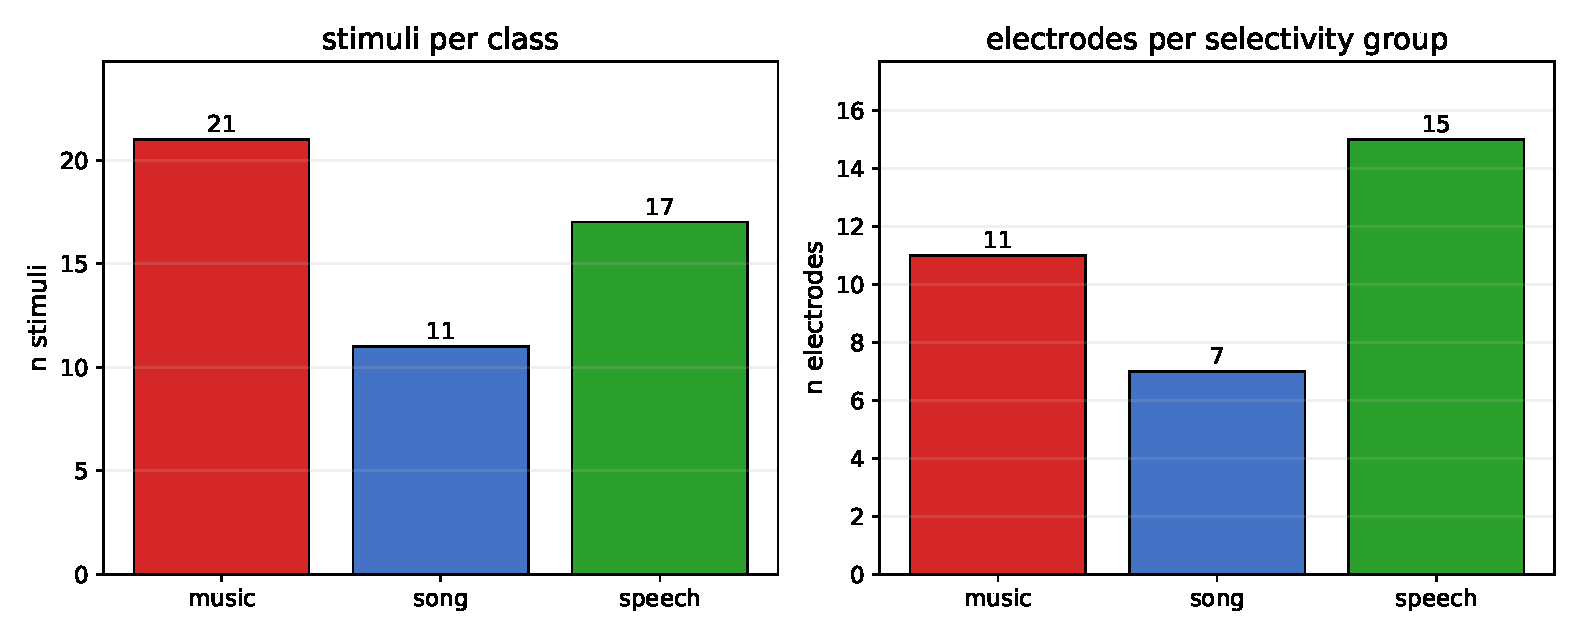
\includegraphics[width=0.72\textwidth]{fig1_dataset_overview.pdf}
\caption{\textbf{Dataset layout.} Stimulus counts per coarse class and electrode counts per selectivity group after trimming to the 49-stimulus \{song, speech, music\} subset. The three subsets used later are \textsf{all} (33 electrodes), \textsf{song\_only} (7 song-selective electrodes), and \textsf{no\_song} (26 speech- and music-selective electrodes); \emph{matched random subsets} are 1000 draws of 7 electrodes from the \textsf{no\_song} pool for a fair size-matched null.}
\label{fig:dataset}
\end{figure}

\subsection{When does the song-vs-music difference appear?}

\emph{We now zoom in on the song-vs-music pair specifically: when during the trial is that distinction actually decodable?} The answer: throughout the trial, at essentially every electrode subset (panel~(b) of Fig.~\ref{fig:mainnorman}). Peak balanced accuracy is 1.00 on \textsf{all} and on the 7 song-selective electrodes (\textsf{song\_only}), and 0.95 on the remaining 26 speech- and music-selective electrodes (\textsf{no\_song}). Peak times differ across subsets: the full pool (\textsf{all}) peaks at $0.47$~s, \textsf{no\_song} at $0.52$~s, and \textsf{song\_only} latest at $0.67$~s, so the seven song-selective contacts lag the 33-electrode pool by $0.20$~s while the 26 non-song contacts sit in between. These timings are consistent with a contribution from early-onset electrodes in the STG onset-vs-sustained spatial map of \citet{Hamilton2018}. The decoder clearly does not depend on song-selective electrodes to reach chance-clearing performance: \textsf{no\_song} still reaches 0.95. Whether \textsf{song\_only} outperforms \textsf{no\_song} in a meaningful way is exactly the question the random-subset control in \S\ref{sec:randsubset} is designed to answer.

\begin{figure}[p]
\centering
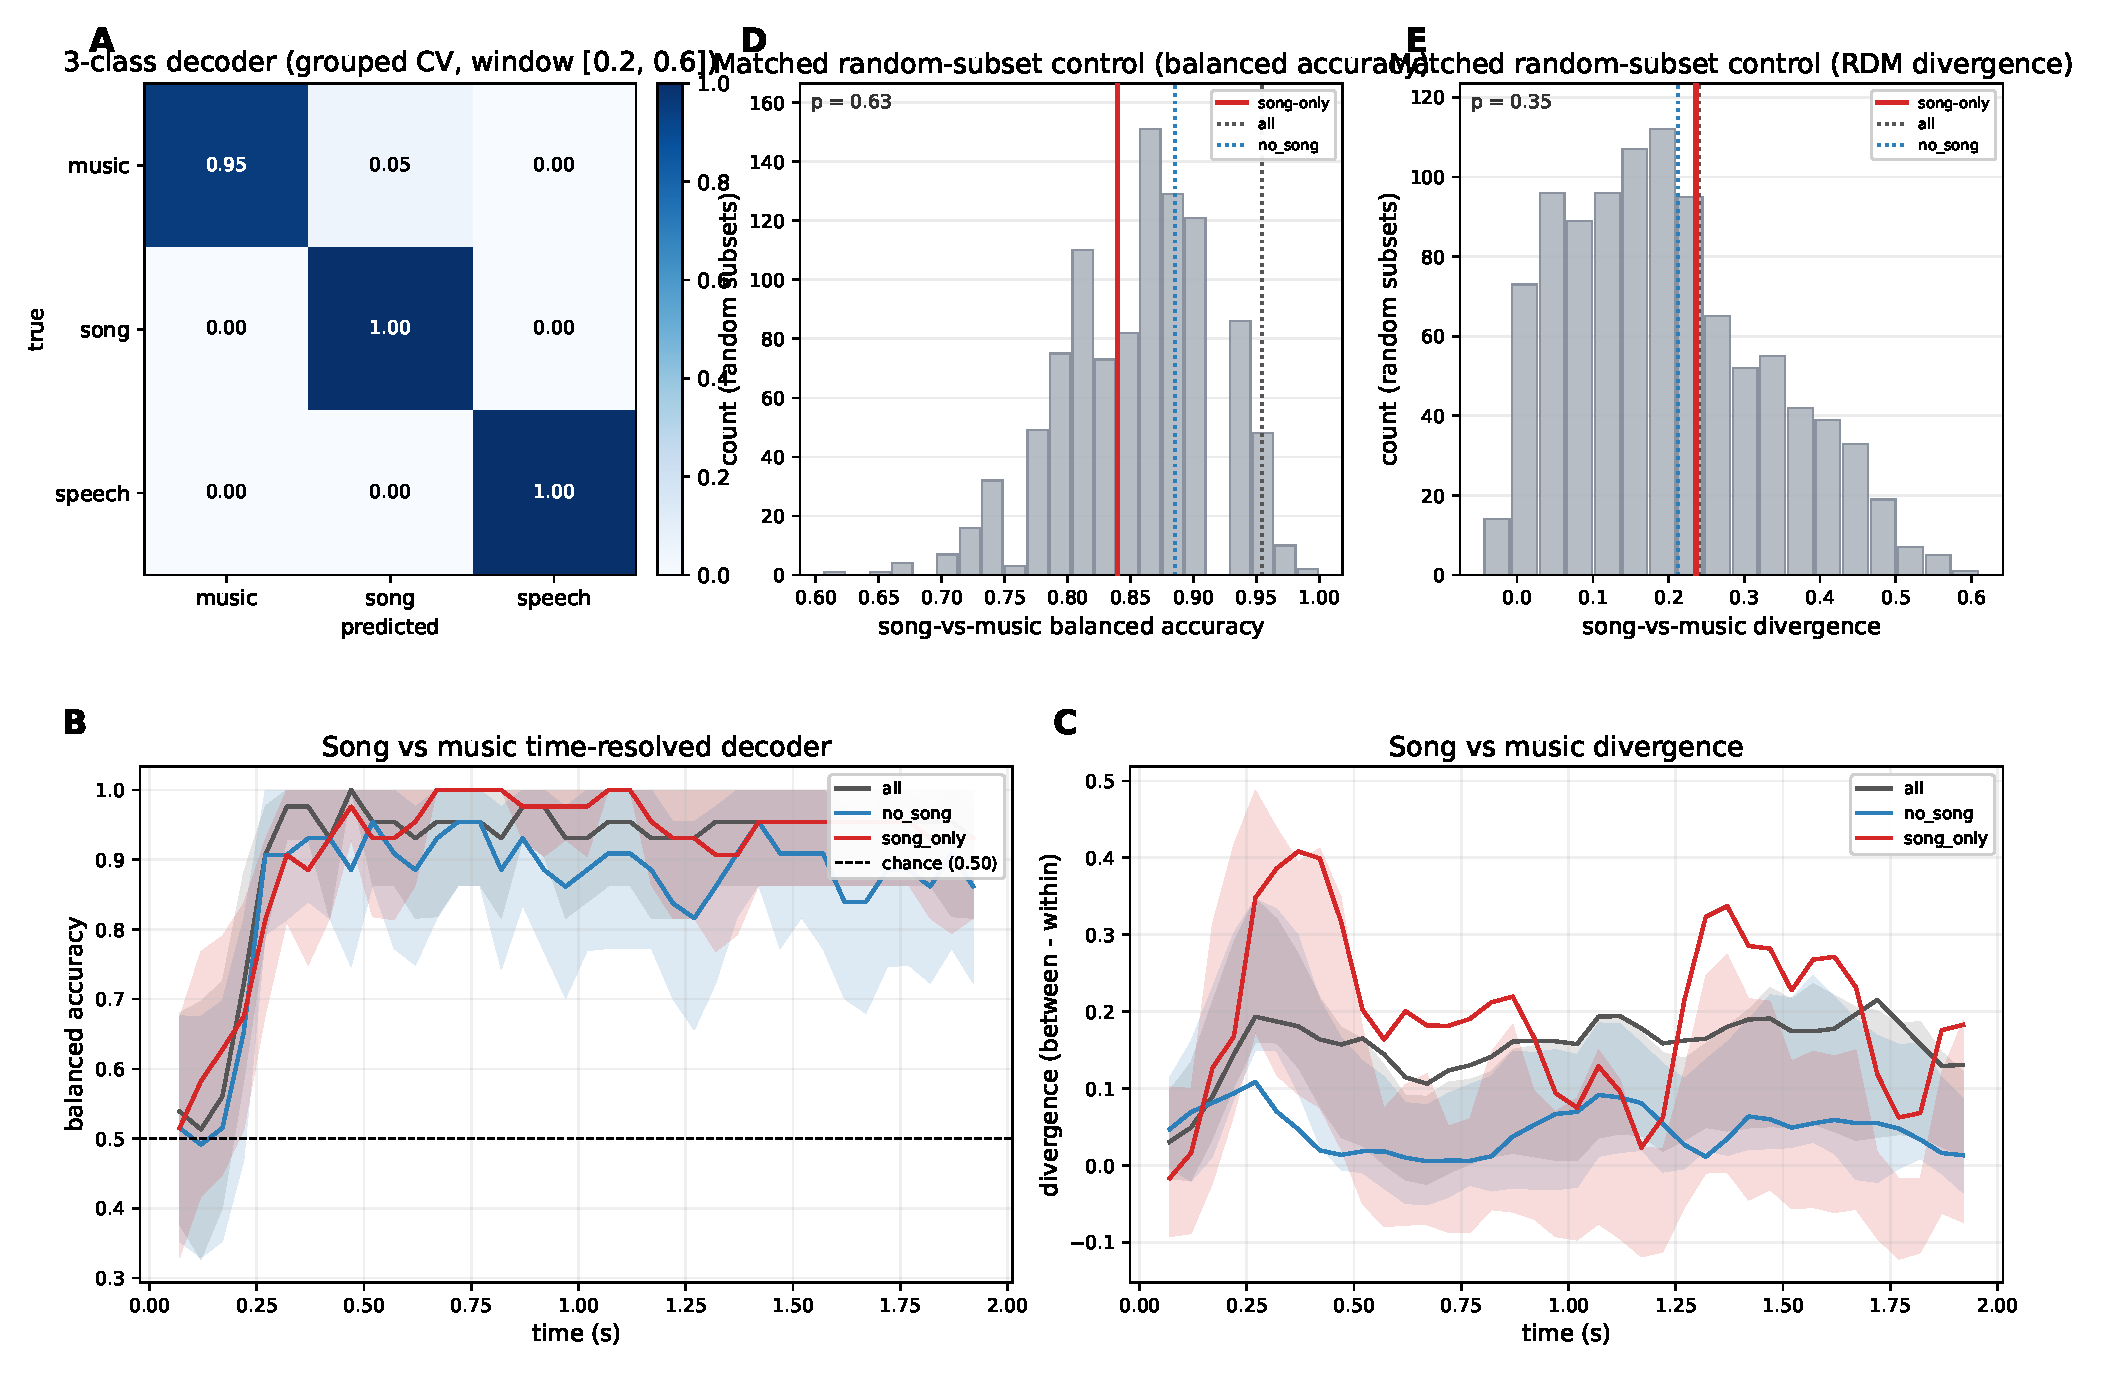
\includegraphics[width=\textwidth]{fig1_main_composite.pdf}
\caption{\textbf{Norman--Haignere decoding, geometry, and matched random-subset null.} \textbf{(a)} Row-normalised confusion matrix for the 3-class logistic-regression decoder (grouped 5-fold CV, early window $[0.2, 0.6]$~s). \textbf{(b)} Time-resolved song-vs-music balanced accuracy (0.15~s sliding windows; shaded: bootstrap 95\% CI; dashed: chance). \textbf{(c)} Classifier-free song-vs-music RDM divergence (same windows; shaded: bootstrap CI). \textbf{(d--e)} Matched random-subset null for balanced accuracy and divergence: grey histograms are 1000 draws of 7 non-song electrodes; red: observed \textsf{song\_only}; reference lines for \textsf{all} and \textsf{no\_song} pools. Empirical one-sided $p$-values vs.\ the random draws are printed on the histograms.}
\label{fig:mainnorman}
\end{figure}

\subsection{Neural separation of song and music}

\emph{Decoding accuracy tells us a classifier can separate the classes. But is the separation also visible in the raw neural geometry, with no classifier involved?} We cross-checked the decoder result with the classifier-free divergence score from \S\ref{sec:methods:divergence}. Every subset produces a divergence curve that rises above the chance-level band (what the score looks like under shuffled labels) within the first 0.3~s (panel~(c) of Fig.~\ref{fig:mainnorman}; Table~\ref{tab:divergence}). Peak divergence is largest for \textsf{song\_only} (0.408, $p_\text{peak} = 0.002$), though it is also the noisiest curve, as expected from only 7 electrodes. \textsf{no\_song} and \textsf{all} peak lower in absolute terms but still clear permutation $p < 0.01$. Song-vs-music structure is therefore present in the neural geometry of every subset, not only in the decoder. As in panel~(b) of Fig.~\ref{fig:mainnorman}, the \textsf{song\_only} curve looks larger than \textsf{all} and \textsf{no\_song}, but the apparent \textsf{song\_only} advantage here is again confounded with subset size; the fair comparison is in \S\ref{sec:randsubset}.

\begin{table}[t]
\centering\small
\caption{\textbf{RDM divergence summary.} Peak divergence, peak time, early-window mean ($[0.2, 0.6]$~s), and permutation $p$-value at peak (1000 shuffles).}
\label{tab:divergence}
\begin{tabular}{lcccc}
\toprule
subset & peak $\divg$ & peak time (s) & early mean $\divg$ & $p_\text{peak}$ \\
\midrule
all        & 0.215 & 1.72 & 0.167 & 0.001 \\
no\_song   & 0.108 & 0.27 & 0.049 & 0.005 \\
song\_only & 0.408 & 0.37 & 0.299 & 0.002 \\
\bottomrule
\end{tabular}
\end{table}

\subsection{Random-subset control: are song-selective electrodes special?}\label{sec:randsubset}

\emph{This is the central question of the paper.} The raw curves in panels~(b--c) of Fig.~\ref{fig:mainnorman} look as if \textsf{song\_only} beats the larger \textsf{no\_song} pool, which would suggest that song-selective electrodes are uniquely informative. But comparing against all 33 electrodes is not a fair test, because smaller electrode sets are easier to decode from. The fair comparison is against other groups of 7 electrodes drawn at random from the non-song pool.

Song-only is not privileged under this fair comparison (panels~(d--e) of Fig.~\ref{fig:mainnorman}). On balanced accuracy the seven song-selective contacts score $0.840$, slightly \emph{below} the mean of the 1000 random seven-electrode draws from the non-song pool ($0.855$; empirical rank $\approx 37$th percentile; one-sided $p = 0.63$ counting how often a random draw meets or beats the song-only score). On RDM divergence the story is not identical: song-only is $0.236$, modestly \emph{above} the random-draw mean ($0.198$; $\approx 65$th percentile; $p = 0.35$). In neither case does the song-only value sit in the extreme upper tail.

The $p$-values implement the same one-sided rule as in \S\ref{sec:methods}: they ask whether song-only is unusually \emph{high} relative to the null. Large $p$ means ``no,'' consistent with no privilege. Separately, a bootstrap on (song-only minus mean null draw) gives a 95\% CI of about $[-0.019,-0.012]$ for balanced accuracy but $[+0.030,+0.047]$ for divergence, so the decoder readout is slightly below the random average while the geometry readout is slightly above it. Both metrics still support the same headline: the seven song-labeled contacts are not a uniquely informative subset compared with other size-matched non-song groups. This is our central negative result: song electrodes as a group do not carry disproportionately more song-vs-music information than neighbouring auditory-cortex electrodes.

\paragraph{Why does song-only appear to beat all-electrodes?} The reason is a size effect, not a selectivity effect. A logistic regression with $k = 7$ features is better conditioned than one with $k = 33$: fewer features, gentler regularisation, lower cross-fold variance. Any random 7-electrode non-song subset gets the same benefit, which is exactly what panels~(d--e) of Fig.~\ref{fig:mainnorman} show. The correct population-level benchmark is therefore the full 33-electrode pool, and the song-only advantage over it is a small-subset ceiling effect.

\paragraph{Are we just measuring the labels?} One might worry that because the song electrodes were defined on the same dataset, our result is circular. This concern is partly mitigated, not fully eliminated. \citet{NormanHaignere2022} derived their labels from the full 165-stimulus task using trial-averaged responses, while our decoder and divergence score are computed on a different object: per-electrode responses to the 49-stimulus $\{$song, speech, music$\}$ subset. So the statistical target is not identical. But the labels are still inherited from the same dataset and same electrodes, so we cannot rule out circularity on principle. The best argument against it here is empirical: if the labels really drove our result, the song electrodes should have sat in the extreme tail of the random-draw distribution. They did not.

\subsection{What remains after controlling for acoustics?}\label{sec:acoustic}

\emph{If song electrodes are not disproportionately informative, the natural follow-up is: what is the decoder picking up on in the first place -- just basic acoustics, or something beyond them?} The acoustic-partialled analysis (\S\ref{sec:methods:acoustic}) answers this by recomputing divergence after subtracting out what is linearly predictable from the cochleogram and spectrotemporal-modulation features. A non-trivial fraction of the song-vs-music signal survives the acoustic subtraction: 33--47\% of the raw peak divergence across the three subsets (panel~(a) of Fig.~\ref{fig:mechanisms}; Table~\ref{tab:acoustic}). Statistically, this surviving structure is borderline. The partialled \textsf{song\_only} peak sits right at the conventional threshold ($p = 0.052$); the other two subsets do not clear it ($p = 0.108$ for \textsf{all}, $p = 0.410$ for \textsf{no\_song}). What we can safely say is narrower than ``post-acoustic code'': some structure remains after regressing out this particular linear acoustic feature set, and the amount that remains is similar across the three subsets. That pattern is in the direction expected for integrative coding in STG \citep{Yi2019,Leonard2024,Sankaran2024} -- i.e., the STG combining acoustic input with higher-order category cues -- but at this sample size and with this feature bank we cannot claim a robustly significant non-acoustic component.
We therefore interpret the residual conservatively: it is not proof of a higher-order song code, but only evidence that this particular linear acoustic feature bank does not explain all of the song-vs-music geometry (the remainder could in principle reflect higher-order auditory structure, nonlinear acoustics, unmodelled vocal timbre, or noise).

\begin{table}[t]
\centering\small
\caption{\textbf{Acoustic partition.} Raw vs acoustic-partialled divergence, fraction of the raw peak that survives partialling, and permutation $p$-values (1000 shuffles, ridge $\lambda=1$, regressors $A_\text{full} \in \mathbb{R}^{49\times 69}$).}
\label{tab:acoustic}
\begin{tabular}{lcccc}
\toprule
subset & peak raw & peak partial & surviving fraction & $p_\text{partial}$ \\
\midrule
all        & 0.215 & 0.088 & 0.395 & 0.108 \\
no\_song   & 0.108 & 0.052 & 0.470 & 0.410 \\
song\_only & 0.408 & 0.191 & 0.331 & 0.052 \\
\bottomrule
\end{tabular}
\end{table}

\begin{figure}[p]
\centering
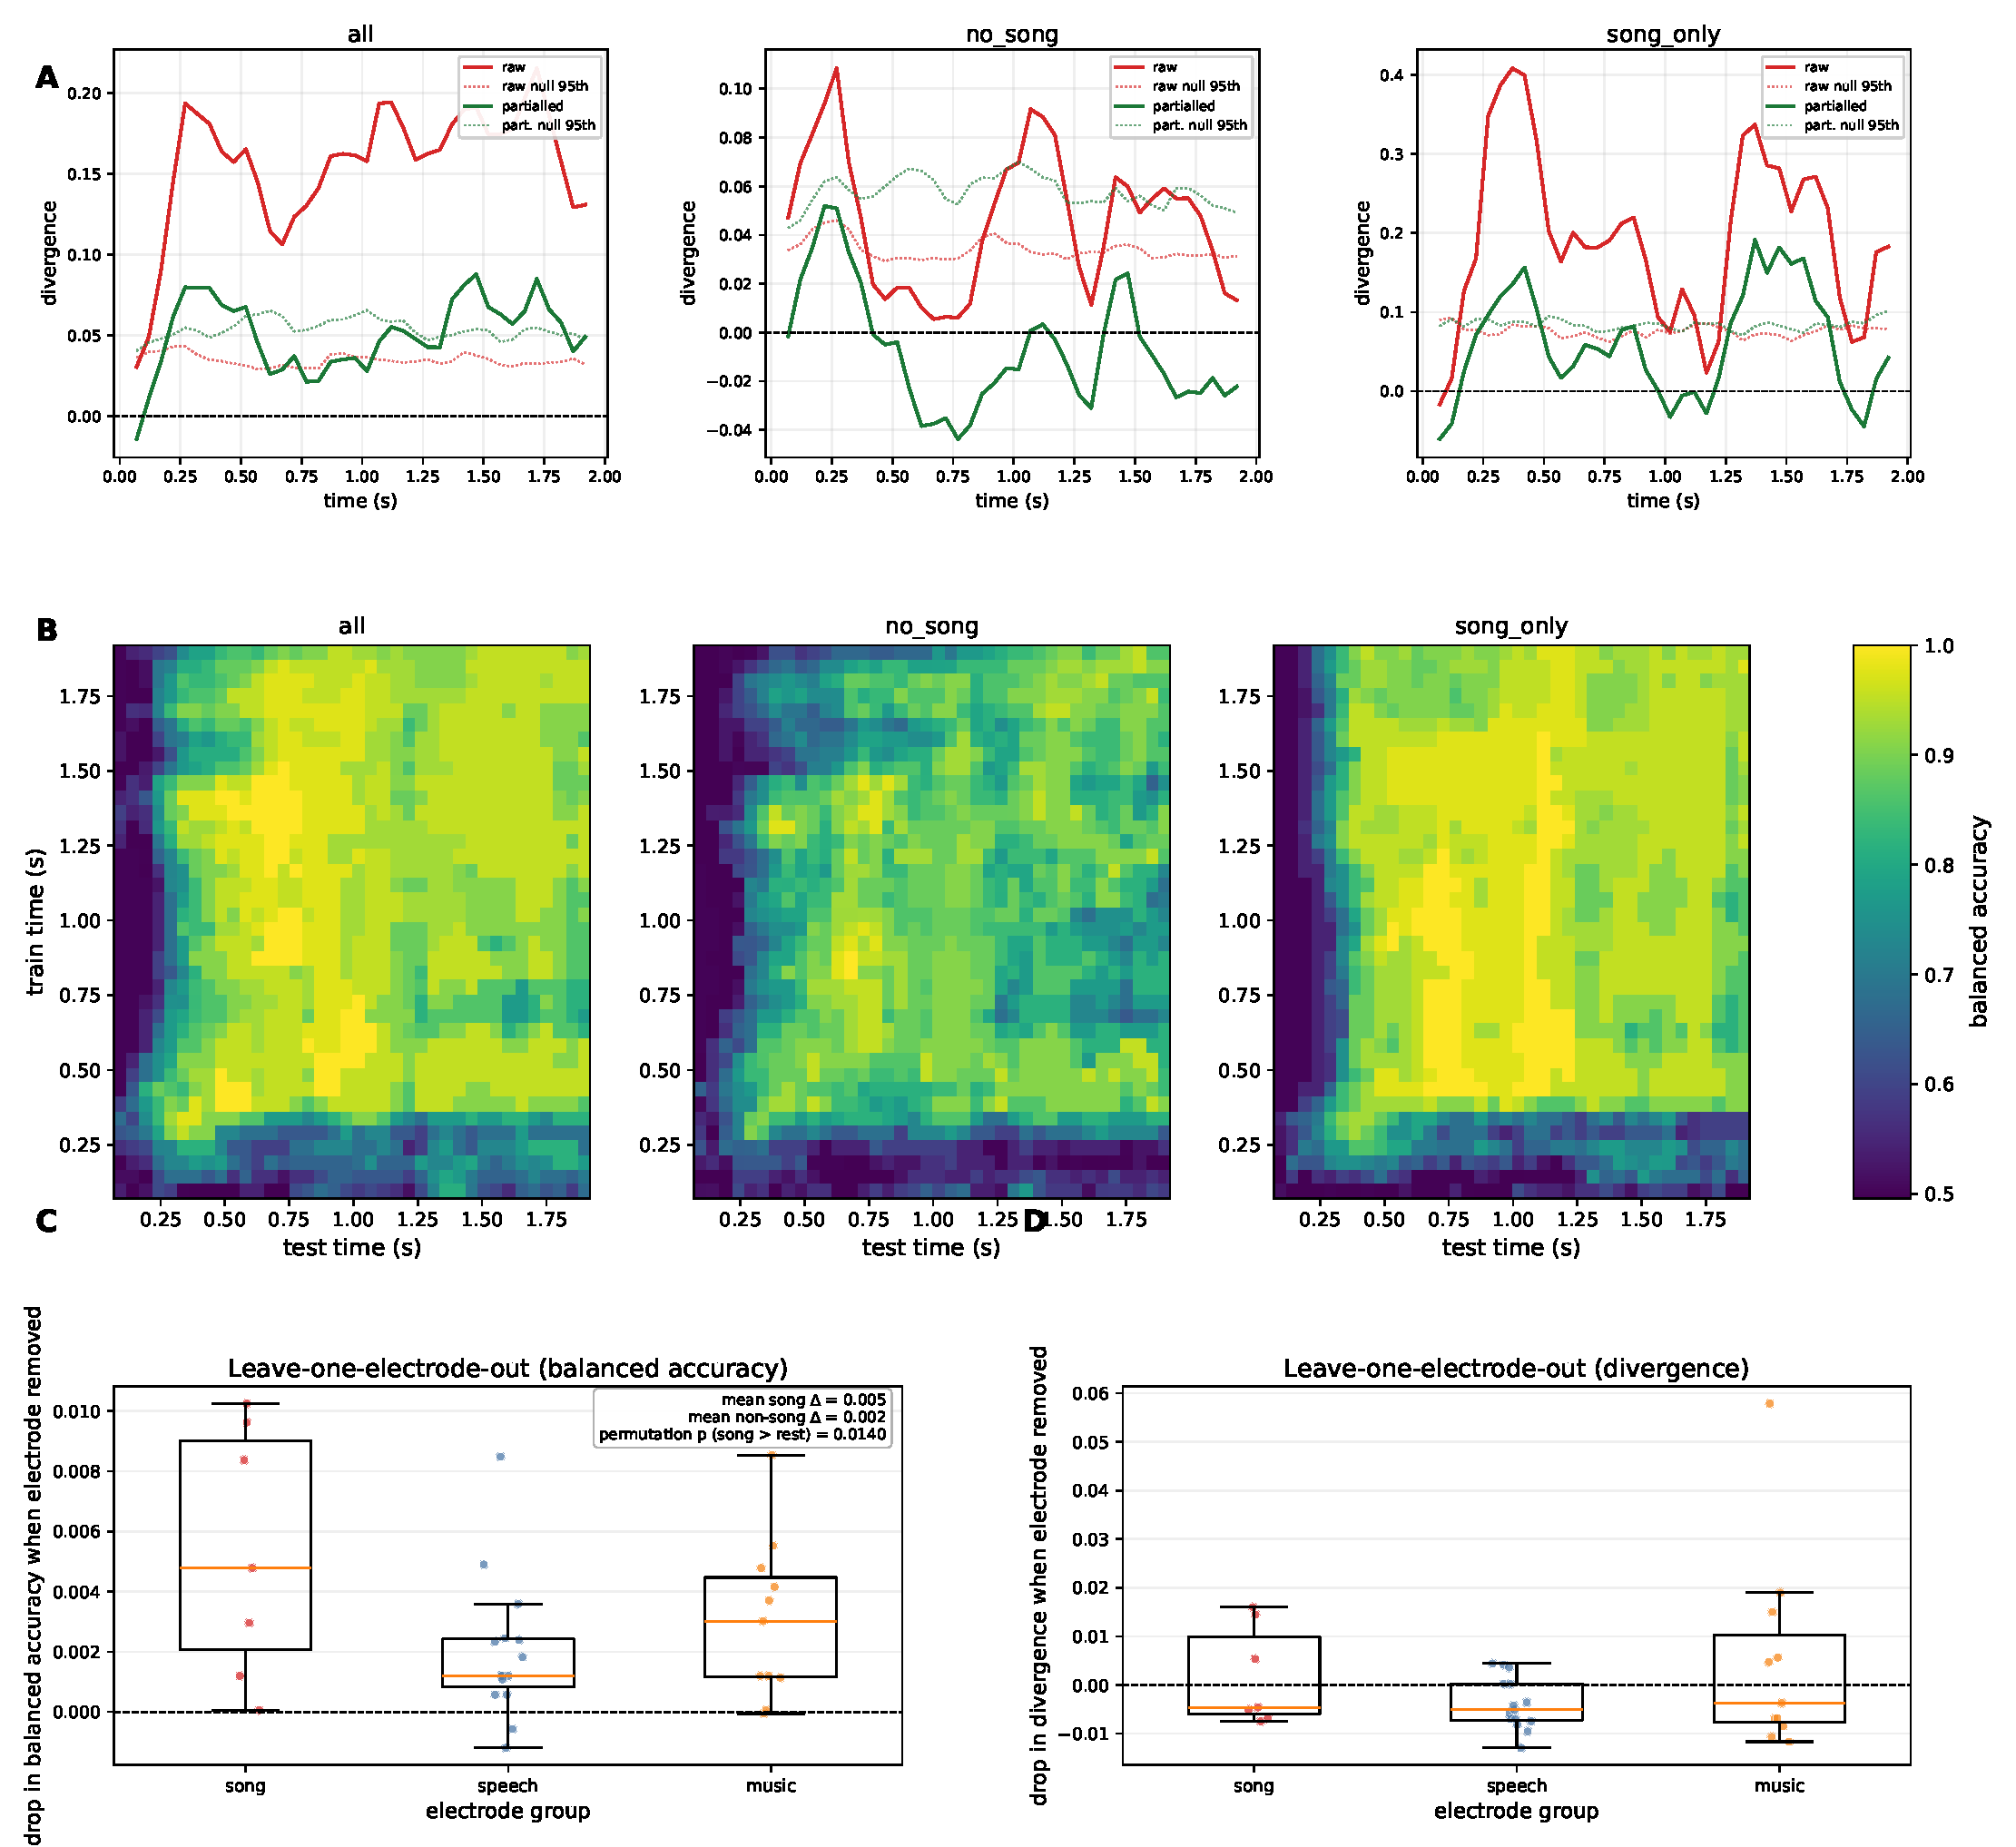
\includegraphics[width=\textwidth]{fig2_mechanisms_composite.pdf}
\caption{\textbf{Mechanistic follow-ups on Norman--Haignere.} \textbf{(a)} Acoustic-partialled divergence: red, raw divergence with label-shuffle 95th-percentile band; green, divergence after ridge-regressing cochleogram + spectrotemporal-modulation features out of the neural features at each window (partialled band refits the regression inside every shuffle). Columns: \textsf{all}, \textsf{no\_song}, \textsf{song\_only}. \textbf{(b)} Cross-temporal generalisation (song vs music): balanced accuracy when training at $t_i$ and testing at $t_j$, shared colour scale across subsets. \textbf{(c--d)} Leave-one-electrode-out change in time-mean balanced accuracy and in early-window divergence; box + jitter by selectivity group; annotation gives group means and permutation $p$ for song $>$ rest on $\Delta$bacc.}
\label{fig:mechanisms}
\end{figure}

\subsection{Temporal stability of the song-vs-music code}\label{sec:tempstab}

\emph{Even if song electrodes are not more informative at peak, they might carry a qualitatively different \textbf{kind} of code: one that stays stable across the trial rather than drifting.} Cross-temporal generalisation tests this: a decoder trained at time $t_i$ is tested at every other time $t_j$, and bright off-diagonals indicate a stable code. A sustained categorical code should generalise across time; a purely onset-driven code should not \citep{Hamilton2018,Holdgraf2017}.

The song-selective subset shows a somewhat more temporally stable representation than the non-song pool (panel~(b) of Fig.~\ref{fig:mechanisms}). Diagonal vs.\ off-diagonal-at-$\geq 0.25$~s balanced accuracy is $0.91/0.84$ for \textsf{all}, $0.91/0.83$ for \textsf{song\_only}, and $0.86/0.76$ for \textsf{no\_song}, so mean off-diagonal accuracy is higher on the seven song contacts than on the 26 non-song contacts ($0.83$ vs.\ $0.76$). We do not have a permutation null on this comparison, so we treat that ordering as descriptive rather than a formal significant result.

\subsection{Per-electrode contributions (leave-one-out)}

\emph{The random-subset control in \S\ref{sec:randsubset} tests song electrodes as a group. Here we run a complementary test at the single-electrode level, asking whether removing any one electrode disproportionately hurts the decoder, and whether those important electrodes concentrate in the song group.} Mean leave-one-out drops in time-mean balanced accuracy are tiny for every selectivity group (panels~(c--d) of Fig.~\ref{fig:mechanisms}; Table~\ref{tab:loo}): $+7.9 \times 10^{-4}$ for song, $+3.5 \times 10^{-4}$ for music, and $-4.1 \times 10^{-4}$ for speech, with a song-vs-rest label permutation $p = 0.23$ on the group-mean contrast (1000 shuffles). Song contacts rank slightly highest on average, but the effect is not distinguishable from chance relabelling, so we do not treat LOO as supporting a second ``special population'' claim: the fair 7-vs-7 matched subset test in \S\ref{sec:randsubset} remains the primary evidence that the seven song contacts as a \emph{set} are not unusually informative relative to other size-matched non-song draws.

\begin{table}[t]
\centering\small
\caption{\textbf{LOO group summary.} Mean drop in time-mean bacc and in early-window $\divg$ when each electrode is removed; permutation $p$ for song-vs-rest on $\Delta$bacc (1000 shuffles).}
\label{tab:loo}
\begin{tabular}{lrrrr}
\toprule
group & $n$ & mean $\Delta$bacc & mean $\Delta\divg$ & $p$ (song vs rest, bacc) \\
\midrule
song   &  7 & $+7.9 \times 10^{-4}$ & $+0.0017$ & 0.23 \\
music  & 11 & $+3.5 \times 10^{-4}$ & $+0.0049$ & -- \\
speech & 15 & $-4.1 \times 10^{-4}$ & $-0.0039$ & -- \\
\bottomrule
\end{tabular}
\end{table}

\subsection{Do more complex models help?}

\emph{A concern with our negative random-subset result is that it might be an artefact of using a linear decoder: maybe a non-linear model could extract much more song-vs-music information from the song electrodes.} Non-linear models do not beat the linear baseline on this dataset (Fig.~\ref{fig:nonlinear}). Neither an RBF-SVM nor an autoencoder-latent + logreg pipeline improves on logistic regression: $\Delta$bacc $= 0$ for song-vs-music; for the three-class task, both alternatives score \emph{below} linear logistic regression ($\Delta$bacc $\approx -0.09$ for the autoencoder pipeline and $\approx -0.03$ for the RBF-SVM). At this sample size and feature dimension, a simple linear decoder already extracts most of the available signal, so adopting a linear decoder throughout the paper does not seem to be leaving obvious non-linear information on the table. This is consistent with the STG literature on low-dimensional feature tuning \citep{Mesgarani2014,Hullett2016}.

\begin{figure}[t]
\centering
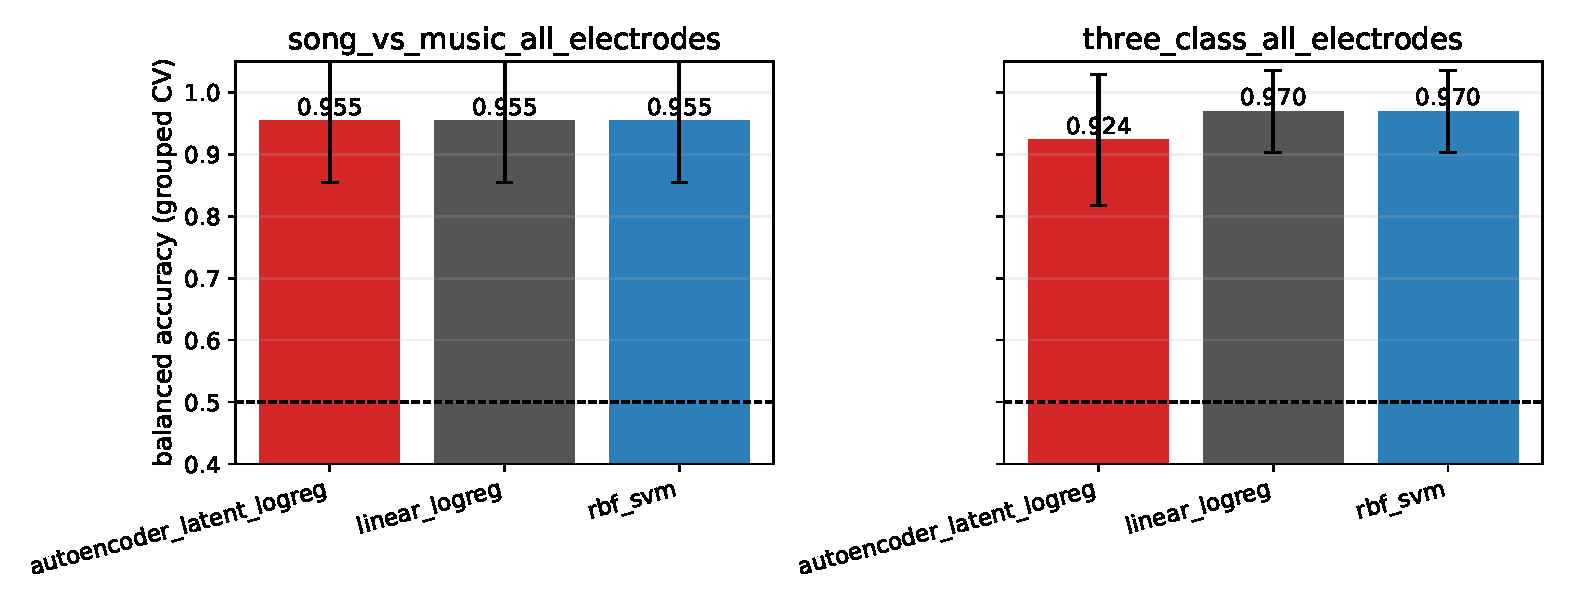
\includegraphics[width=0.9\textwidth]{fig_nonlinear_comparison.pdf}
\caption{\textbf{Non-linear supplement.} Grouped CV balanced accuracy of three model families on two tasks (three-class and song-vs-music, all-electrodes) using identical stimulus-grouped 5-fold splits. Error bars are across-fold standard deviations. Song-vs-music matches the linear baseline; on the three-class task both non-linear pipelines trail logistic regression.}
\label{fig:nonlinear}
\end{figure}

\subsection{Does the result hold in continuous music?}

\emph{So far we have shown that song-vs-music structure is decodable and visible in geometry for every Norman subset, but the seven song-selective contacts are not privileged under a fair 7-vs-7 draw; that much of the signal overlaps our acoustic feature bank, with a suggestive partialled residual; and that non-linear decoders do not overturn the linear picture on Norman. We next ask whether the same qualitative story---strong decodability without a privileged anatomical subset---holds in continuous, naturalistic music using \citet{Bellier2023}.} Table~\ref{tab:bellier} reports the vocal-vs-instrumental decoder on the 2395-electrode cross-patient supergrid defined in \S\ref{sec:methods:bellier}. The interleaved-folds fix was essential: with naive contiguous folds, folds 3 and 4 of a 5-fold split fall entirely in the instrumental region and balanced accuracy is undefined.

\begin{table}[t]
\centering\small
\caption{\textbf{Bellier (2023) vocal-vs-instrumental decoder.} $1903$ windows, 500~ms / 100~ms, interleaved 5-fold blocked-time CV. CNN is run only on subsets where logreg clears chance by $\geq 0.05$. Column $n_\text{CNN}$ is the number of electrodes fed to the CNN (256 when the subset is larger, else the full count).}
\label{tab:bellier}
\begin{tabular}{lrrrrrr}
\toprule
subset & $n_\text{LR}$ & logreg bacc & logreg AUC & $n_\text{CNN}$ & CNN bacc & CNN AUC \\
\midrule
all        & 2395 & \textbf{0.777} & 0.899 & 256 & 0.768 & 0.839 \\
right\_STG &  181 & 0.692 & 0.814 & 181 & \textbf{0.730} & 0.838 \\
left\_STG  &  245 & 0.684 & 0.780 & 245 & 0.727 & 0.807 \\
non\_STG   & 1969 & 0.730 & 0.892 & 256 & 0.732 & 0.825 \\
\bottomrule
\end{tabular}
\end{table}

\begin{figure}[p]
\centering
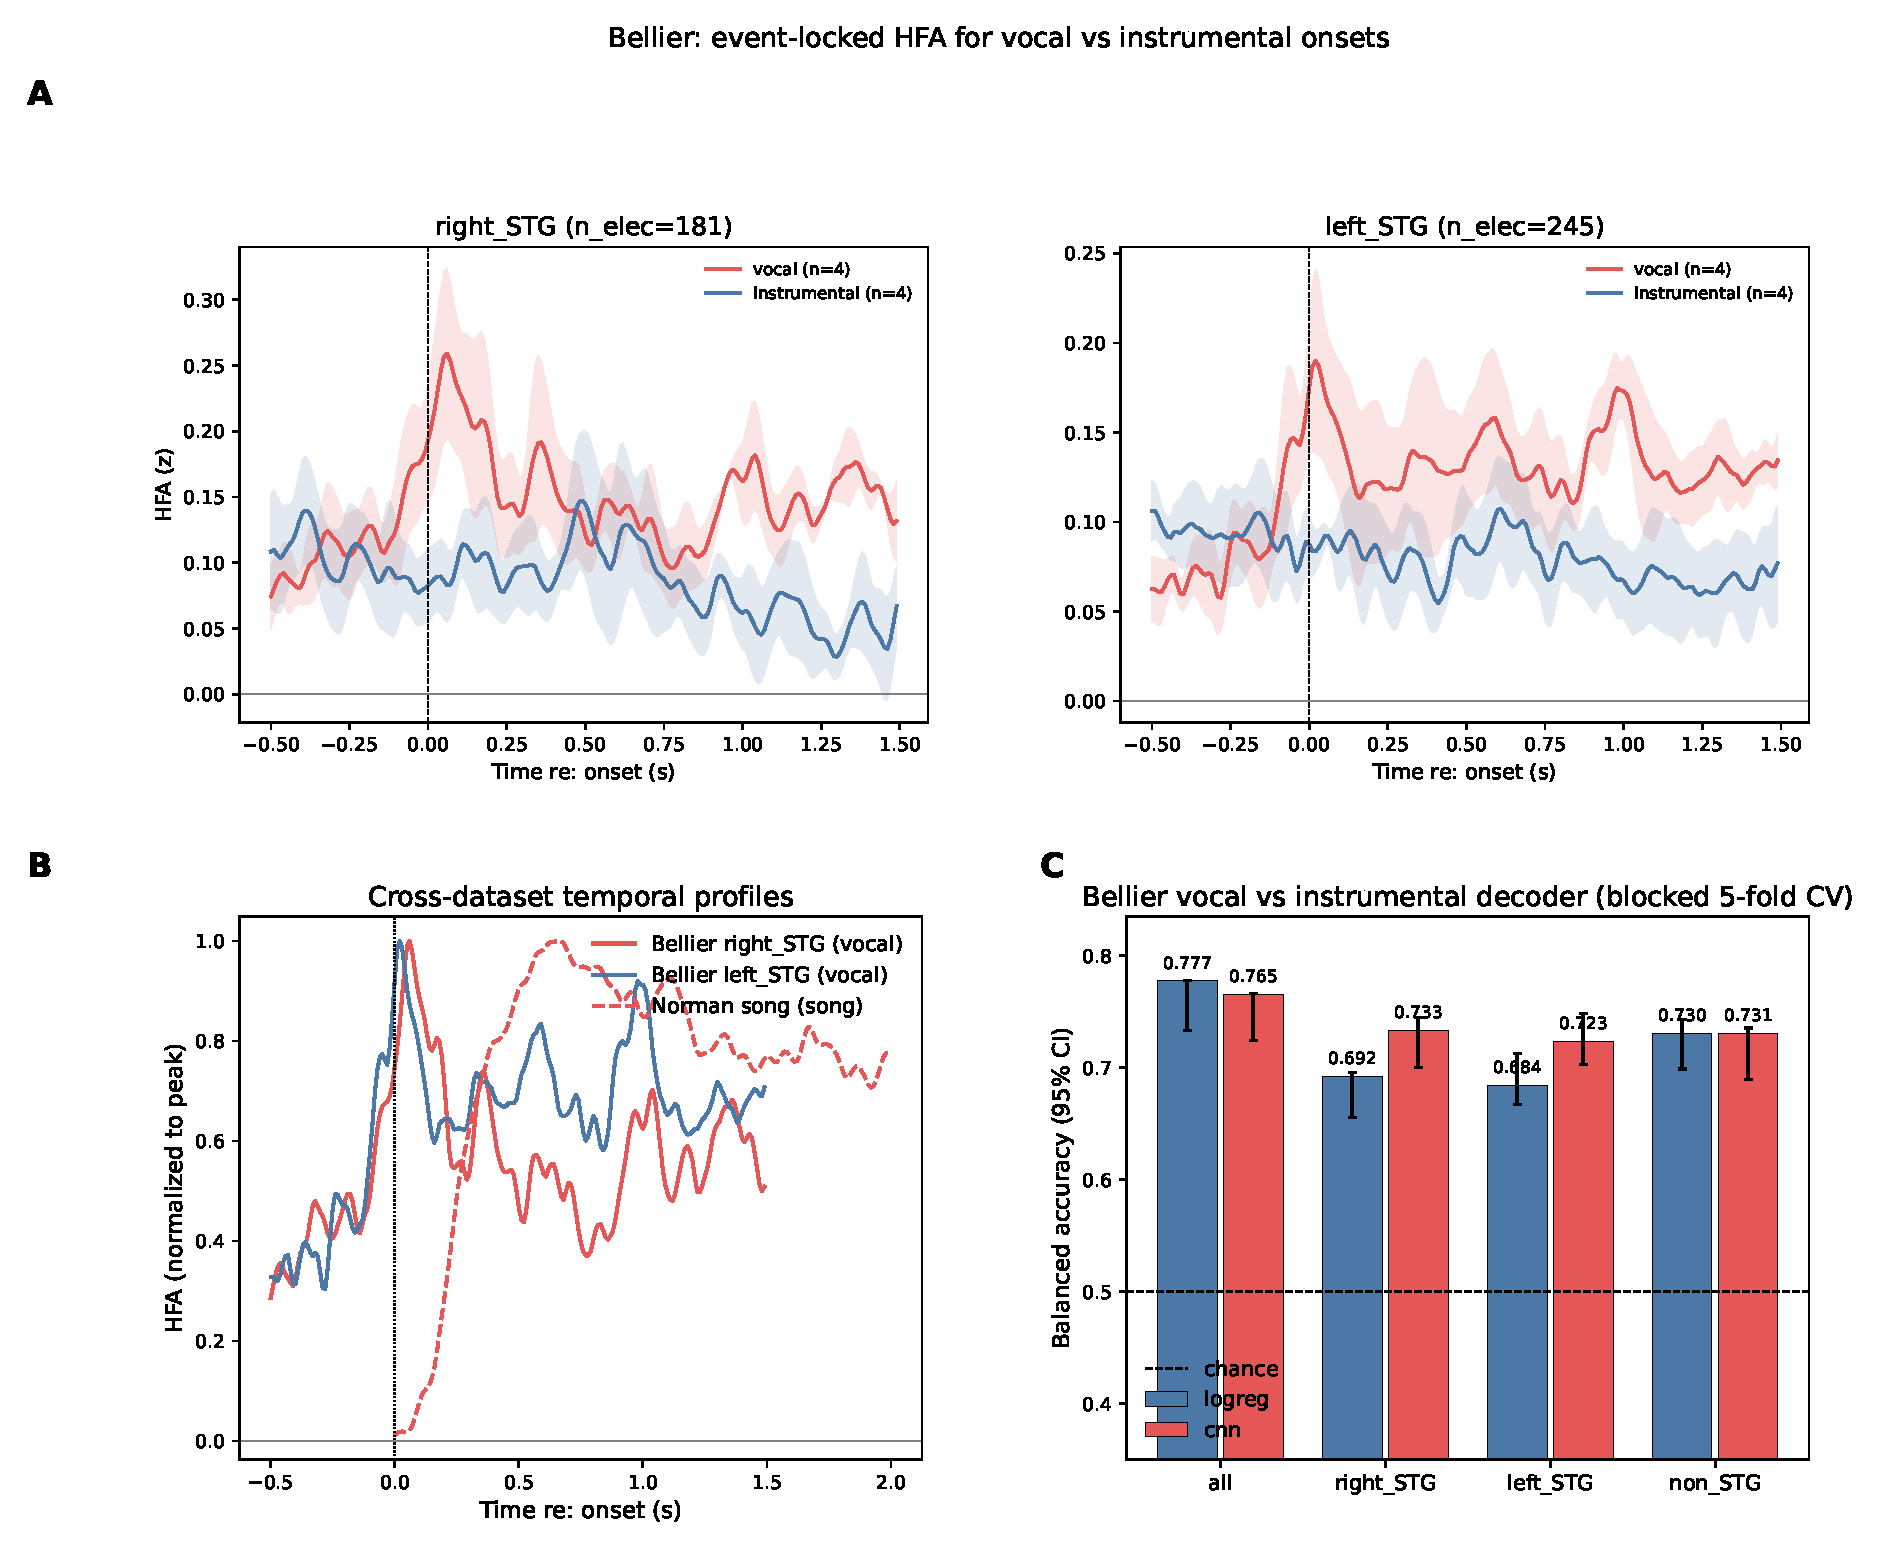
\includegraphics[width=\textwidth]{fig3_bellier_composite.pdf}
\caption{\textbf{Bellier extension and cross-dataset profiles.} \textbf{(a)} Event-locked mean HFA (SEM band) at vocal and instrumental onsets for right and left STG ($n = 4$ onset events per condition after the event detector). \textbf{(b)} Peak-normalised overlay: Bellier STG at vocal onsets vs.\ Norman song-electrode responses on song trials (shape comparison only; different normalisations and locking). \textbf{(c)} Vocal-vs-instrumental decoder: mean balanced accuracy with 95\% bootstrap CI for logistic regression and TinyTemporalCNN (Table~\ref{tab:bellier}).}
\label{fig:bellierwhole}
\end{figure}

Two findings stand out in Table~\ref{tab:bellier} and panel~(c) of Fig.~\ref{fig:bellierwhole}. First, right STG slightly beats left STG on both logreg and CNN, going in the same direction as the right-hemispheric vocal bias reported by \citet{Bellier2023}. The absolute difference is small ($0.692$ vs.\ $0.684$ on logreg), and we did not run a permutation null for this subset comparison, so we treat this as a directional replication rather than a formally significant finding. Second, the whole-pool bar is the highest overall, consistent with distributed rather than STG-exclusive coding. Relative to window-mean logistic regression, the CNN adds roughly three to four bacc points on the STG subsets, whereas on \textsf{all} and \textsf{non\_STG} the two models stay within a few tenths of a point (with the CNN limited to 256 contacts), so the extra temporal modelling appears concentrated in STG.

\subsection{Comparing response shapes across datasets}

\emph{The Bellier decoder shows the vocal-vs-instrumental distinction is decodable, but it does not tell us how the underlying response looks over time. We now compare the shape of that response against Norman to see whether the two datasets are emphasising the same or different phases of the HFA.} We compared HFA profiles on response shape only, not amplitude (panels~(a--b) of Fig.~\ref{fig:bellierwhole}). The cleanest summary is the onset-sustained ratio (Table~\ref{tab:profiles}). Bellier right\_STG at vocal onsets is transient (ratio $1.57$), Bellier left\_STG is balanced ($1.11$), and Norman \textsf{song} electrodes at song trials are strongly sustained ($0.11$), which is the most sustained response in the table. The two datasets sample different phases of the response: Bellier highlights a short onset transient while Norman highlights a long sustained phase.

\begin{table}[h]
\centering\small
\caption{\textbf{Temporal-profile features (selected).} Peak latency, onset-sustained ratio (mean $[0,0.2]$/mean $[0.5,1.5]$; $< 1$ = sustained), and trapezoidal AUC in $[0,1.5]$. Lower rows: Norman group $\times$ stimulus class.}
\label{tab:profiles}
\begin{tabular}{llrrrr}
\toprule
dataset & profile & peak $t$ (s) & onset/sustained & AUC \\
\midrule
Bellier & right\_STG @ vocal        & 0.06 & 1.57 & 0.23 \\
Bellier & right\_STG @ instrumental & 0.49 & 1.30 & 0.12 \\
Bellier & left\_STG  @ vocal        & 0.02 & 1.11 & 0.20 \\
Norman  & song-elec  @ song         & 0.66 & \textbf{0.11} & 100.75 \\
Norman  & song-elec  @ music        & 0.40 & 0.44 & 34.72 \\
Norman  & music-elec @ music        & 0.37 & 0.43 & 82.08 \\
Norman  & speech-elec @ speech      & 0.35 & 0.49 & 122.41 \\
\bottomrule
\end{tabular}
\end{table}

This shape mismatch is expected given how differently the stimuli are presented. Norman's 2-second clip paradigm trial-locks responses, which averages in the sustained post-onset phase; Bellier's event-locking at vocal onsets inside a continuous song samples mostly the transient at stimulus change. The sustained song-tracking shape is clearly visible in Norman song electrodes, but it is not the first-order phenomenon at Bellier's right-STG vocal onsets. For our central claim (song electrodes are informative but not privileged), this matters because it shows the claim does not depend on a specific paradigm: both the trial-locked and the event-locked view return a decodable signal that is distributed rather than concentrated in any one anatomical subset.

\FloatBarrier
% =============================================================================
\section{Discussion}\label{sec:discussion}
% =============================================================================

\paragraph{How this refines \citet{NormanHaignere2022}.} The original paper showed that song-selective electrodes exist in the sense that their trial-averaged response is larger for song than for other sounds. Our re-analysis asks a slightly different question: are those same electrodes disproportionately \emph{informative} for a decoder trying to separate song from instrumental music? An electrode can fire more strongly during song without actually helping a classifier, so the two questions are not the same. The answer we get is: no, under the primary matched 7-vs-7 random-subset test. A song-selective electrode fires more strongly to song on average, but the seven song contacts as a set do not sit in the extreme tail of size-matched non-song draws. The song electrodes do show one secondary pattern: their representation looks somewhat more temporally stable (Fig.~\ref{fig:mechanisms}, panel~b). A leave-one-out check on time-mean decoding does not yield a significant song-vs-rest group contrast ($p \approx 0.23$). Neither overturns the group-level null. The specialisation reported in \citet{NormanHaignere2022} is real and consistent with our data; it is just narrower than a naive reading would suggest.

\paragraph{Acoustic vs. post-acoustic coding.} Subtracting out low-level acoustic information from the neural features removes about two-thirds of the song-vs-music RDM peak but leaves a residual (fraction surviving $0.33$--$0.47$). Most of what the brain is doing in this distinction, then, really is just tracking basic sound structure. The permutation test on the residual does not cleanly clear significance at this $N$: $p = 0.052$ for \textsf{song\_only}, $p = 0.108$ for \textsf{all}, $p = 0.410$ for \textsf{no\_song}. We therefore cannot claim a robustly significant non-acoustic component, and we should not call the surviving structure a ``post-acoustic code.'' What we can say is that some geometry remains after regressing out the specific linear acoustic feature set of \citet{NormanHaignere2022}, that the surviving fraction is similar across subsets, and that the partialled peak arrives later in the trial ($1.37$--$1.47$~s, compared to raw peaks at $0.37$--$1.72$~s). These are the directions expected if the STG combines basic acoustic input with higher-order category cues \citep{Hullett2016,BhayaGrossman2022,Mesgarani2014,Yi2019,Leonard2024,Sankaran2024}, but they are suggestive rather than conclusive.

\paragraph{Does it hold in continuous music?} The Bellier extension plays two roles. First, it is a naturalistic sanity check \citep{HamiltonHuth2020}: a vocal-vs-instrumental decoder reaches $0.78$ balanced accuracy on 191~s of continuous song, and right STG slightly beats left STG in the same direction as \citet{Bellier2023} (we did not run a permutation null on the anatomical comparison, so this is directional only). Second, the cross-dataset temporal-profile comparison shows that the two datasets emphasise different phases of the response. Norman's trial-locked profiles highlight the sustained phase, while Bellier's vocal-onset profiles highlight the transient onset. The ``song-tracking'' effect visible in \citet{NormanHaignere2022}'s 2-second clips is therefore best understood as a sustained post-onset response rather than a short onset transient. The two paradigms sample different halves of the same underlying response, which is expected given how differently the stimuli are presented.

\paragraph{Caveats.}
(i) \emph{Sample size.} 33 Norman electrodes and 49 stimuli is small. Our partialled-divergence $p$-values sit near $0.05$ because $N$ is modest, not because the effect is obviously tiny. The signed direction and subset ordering are stable across bootstraps and shuffles; the absolute significance is under-powered.
(ii) \emph{Acoustic feature bank.} We partial out the exact regressors \citet{NormanHaignere2022} use. Richer audio embeddings (e.g.\ HuBERT, self-supervised music encoders) would absorb more of the raw signal, so our surviving fraction is a conservative upper bound on the non-acoustic residual.
(iii) \emph{No permutation null on several Bellier comparisons.} We do not have a permutation null on the Bellier balanced-accuracy numbers or on the cross-temporal-generalisation stability gap in \S\ref{sec:tempstab}. The right-vs-left-STG ordering and the ``more stable code on song electrodes'' observation are therefore directional rather than formally significant. Adding these nulls is the single most fixable gap in the paper and is listed in Future Directions.
(iv) \emph{Song-electrode labels are author-supplied and defined on the same dataset.} We inherit the component assignments from \citet{NormanHaignere2022} rather than re-deriving them on held-out stimuli. The matched random-subset control does not require the labels to be ``correct,'' and the null result cannot be driven by the labels being informative -- if they were, the song electrodes would sit in the upper tail of the random-draw distribution rather than near its middle. But a noisy or mis-specified label set could also produce the same null. A stronger follow-up would be to re-derive song-selectivity on a held-out stimulus split and then apply the random-subset control on the out-of-sample labels.

\paragraph{Future directions.} Four natural next steps, in rough order of payoff for the effort required:
(i) add label-shuffle permutation nulls to the Bellier decoder (for both the overall bacc and the right-vs-left-STG subset comparison) and to the cross-temporal generalisation gap; this is the cheapest upgrade that would turn several currently directional claims into formally significant ones;
(ii) re-derive song-selectivity on a held-out stimulus split and re-apply the random-subset control on the out-of-sample labels, which would close the residual circularity in Caveat (iv);
(iii) replace the acoustic regressor bank with a modern self-supervised audio embedding to push the surviving-fraction estimate in \S\ref{sec:acoustic} closer to its true upper bound;
(iv) apply the partialled-divergence pipeline to the Bellier stimulus windows to ask whether the sustained vocal-tracking component that emerges in the continuous song also survives acoustic partialling.

\paragraph{Novelty.} Our contributions on top of the published work are the matched random-subset control, the acoustic-partialled divergence pipeline, and the cross-dataset temporal-profile comparison (together with the interleaved-blocked-folds CV fix on Bellier). Taken together, these test whether the ``song-selective population exists'' result also implies disproportionate information content, and find that it does not.

\paragraph{Selectivity versus information.}
More broadly, our result illustrates why response selectivity and information privilege should be treated as separate claims. A neural site can respond more strongly to a category without being an unusually strong channel for decoding that category at fixed electrode count. In ECoG work, small labelled groups can look impressive when compared against a much larger pool even when size-matched controls would show similar decodability. Future claims about category-selective populations should therefore pair response-amplitude or component-based selectivity with size-matched information controls, not only with contrasts against the full grid.

\paragraph{Code and data availability.} All analyses run from the repository root: \path{python logic/pipeline.py} (random seed 42) or \path{python scripts/generate_composite_figures.py} for the multi-panel figures (see \path{--help}, including \path{--only 3} for the Bellier composite alone). The full codebase, including \path{neuro120_main_reproduction.ipynb} (full write-up reproduction) and \path{neuro120_bellier_supplement.ipynb} (Bellier extension and supplementary figures), is available at \url{https://github.com/djordjeivanovic11/neuro120-project}. A separate document states course policy on generative-AI use. Norman--Haignere data are from the public release accompanying \citet{NormanHaignere2022}; Bellier ECoG data are from the public release accompanying \citet{Bellier2023}.

% =============================================================================
\clearpage
\begin{thebibliography}{99}
\small
\bibitem[Bellier et al.(2023)]{Bellier2023}
Bellier, L., Llorens, A., Marciano, D., Gunduz, A., Schalk, G., Brunner, P., \& Knight, R.\ T. (2023).
\emph{Music can be reconstructed from human auditory cortex activity using nonlinear decoding models.}
PLOS Biology, 21(8), e3002176.

\bibitem[Bhaya-Grossman \& Chang(2022)]{BhayaGrossman2022}
Bhaya-Grossman, I., \& Chang, E.\ F. (2022).
\emph{Speech computations of the human superior temporal gyrus.}
Annual Review of Psychology, 73, 79--102.

\bibitem[Hamilton et al.(2018)]{Hamilton2018}
Hamilton, L.\ S., Edwards, E., \& Chang, E.\ F. (2018).
\emph{A spatial map of onset and sustained responses to speech in the human superior temporal gyrus.}
Current Biology, 28(12), 1860--1871.e4.

\bibitem[Hamilton \& Huth(2020)]{HamiltonHuth2020}
Hamilton, L.\ S., \& Huth, A.\ G. (2020).
\emph{The revolution will not be controlled: natural stimuli in speech neuroscience.}
Language, Cognition and Neuroscience, 35(5), 573--582.

\bibitem[Holdgraf et al.(2017)]{Holdgraf2017}
Holdgraf, C.\ R., Rieger, J.\ W., Micheli, C., Martin, S., Knight, R.\ T., \& Theunissen, F.\ E. (2017).
\emph{Encoding and decoding models in cognitive electrophysiology.}
Frontiers in Systems Neuroscience, 11, 61.

\bibitem[Hullett et al.(2016)]{Hullett2016}
Hullett, P.\ W., Hamilton, L.\ S., Mesgarani, N., Schreiner, C.\ E., \& Chang, E.\ F. (2016).
\emph{Human superior temporal gyrus organization of spectrotemporal modulation tuning derived from speech stimuli.}
Journal of Neuroscience, 36(6), 2014--2026.

\bibitem[Leonard et al.(2024)]{Leonard2024}
Leonard, M.\ K., Gwilliams, L., Sellers, K.\ K., Chung, J.\ E., Xu, D., Mischler, G., Mesgarani, N., Welkenhuysen, M., Dutta, B., \& Chang, E.\ F. (2024).
\emph{Large-scale single-neuron speech sound encoding across the depth of human cortex.}
Nature, 626, 593--602.

\bibitem[Mesgarani et al.(2014)]{Mesgarani2014}
Mesgarani, N., Cheung, C., Johnson, K., \& Chang, E.\ F. (2014).
\emph{Phonetic feature encoding in human superior temporal gyrus.}
Science, 343(6174), 1006--1010.

\bibitem[Norman-Haignere et al.(2015)]{NormanHaignere2015}
Norman-Haignere, S., Kanwisher, N.\ G., \& McDermott, J.\ H. (2015).
\emph{Distinct cortical pathways for music and speech revealed by hypothesis-free voxel decomposition.}
Neuron, 88(6), 1281--1296.

\bibitem[Norman-Haignere et al.(2022)]{NormanHaignere2022}
Norman-Haignere, S.\ V., Feather, J., Boebinger, D., Brunner, P., Ritaccio, A., McDermott, J.\ H., Schalk, G., \& Kanwisher, N. (2022).
\emph{A neural population selective for song in human auditory cortex.}
Current Biology, 32(7), 1470--1484.e12.

\bibitem[Sankaran et al.(2024)]{Sankaran2024}
Sankaran, N., Leonard, M.\ K., Theunissen, F.\ E., \& Chang, E.\ F. (2024).
\emph{Encoding of melody in the human auditory cortex.}
Science Advances, 10(13), eadk0010.

\bibitem[Yi et al.(2019)]{Yi2019}
Yi, H.\ G., Leonard, M.\ K., \& Chang, E.\ F. (2019).
\emph{The encoding of speech sounds in the superior temporal gyrus.}
Neuron, 102(6), 1096--1110.
\end{thebibliography}

% =============================================================================
\clearpage
\appendix

\section*{Appendix A: Project Breakdown}
\addcontentsline{toc}{section}{Appendix A: Project Breakdown}

\sloppy
Below we summarise who led which parts of the project. The repository (\texttt{logic/}, notebooks under the project root, and \texttt{results/}) is the ground truth for specific modules and figures.

\paragraph{Djordje Ivanovic.}
Djordje implemented and maintained most of the codebase: end-to-end orchestration in \texttt{logic/pipeline.py}, caching and configuration, the main and Bellier supplement notebooks, and the scripts that regenerate tables and composite figures. He ran the headline analyses (matched random-subset null, acoustic partialling, cross-temporal matrices, LOO, Bellier decoder and profiles, nonlinear controls) and drafted Methods (\S\ref{sec:methods}), Results (\S\ref{sec:results}), and the bulk of the Discussion (\S\ref{sec:discussion}). He also handled GitHub maintenance and release hygiene so the project stays reproducible for graders.

\paragraph{Georgia Hutchinson.}
Georgia took the lead on explaining the statistical pipeline and analysis choices in plain language: how cross-validation is grouped, what the nulls test, and how to read the main figures without overstating. She worked closely with Djordje to align those explanations with the actual code paths and outputs. She contributed to validating the core Norman decoding setup, polishing presentation of results, and tightening captions and tables so they match the numbers in \texttt{results/tables/}.

\paragraph{JaKayla Harris.}
JaKayla led the literature survey that frames the Introduction (\S\ref{sec:intro}): prior work on auditory selectivity, how it connects to Norman--Haignere and Bellier, and careful handling of citations and bibliography formatting. She participated in group ideation on motivating questions and plausible follow-ups once the null results were clear, and helped keep the narrative accessible to a non-specialist reader.

\paragraph{Joint work.}
All three members scoped the research questions together, agreed on the matched random-subset control and the acoustic-partialled extension, integrated peer-review feedback, and reviewed every figure, table, and headline number before submission.

% =============================================================================
\section*{Appendix B: AI Use}
\addcontentsline{toc}{section}{Appendix B: AI Use}

\sloppy
This appendix documents how generative AI was used in the project, what we verified ourselves, and where suggestions shaped the write-up. We did not use AI to invent results; numbers in the paper come from the pipeline output in \texttt{results/tables/*.csv}.

\paragraph{Tools used.}
\begin{itemize}
\setlength{\itemsep}{1pt}
    \item \emph{Cursor (IDE).} Plotting code and figures for the write-up; comments and \texttt{README} for setup and reproduction; help with caching, threading, and local GPU use; tidier structure (\texttt{config}, \texttt{data\_utils}); minor LaTeX figure layout.
    \item \emph{Modeling and reading.} Stress-testing assumptions; summarizing papers we had not read end-to-end and pointing to pages and figures that mattered for our analyses.
    \item \emph{Writing support.} Grammar and clarity; checks that we were not misrepresenting or overstating results. One concrete example: we briefly considered an autoencoder for a three-class problem already handled well by logistic regression; the model echoed our sense that adding it would not help the claims we actually wanted to make. We also used AI to draft this appendix and to spot-check citations.
\end{itemize}

\paragraph{What we verified ourselves.}
\begin{itemize}
\setlength{\itemsep}{1pt}
    \item We interpreted accuracies, model behavior, and follow-up questions ourselves, grounded in the outputs.
\end{itemize}

\paragraph{What misled us once.}
\begin{itemize}
\setlength{\itemsep}{1pt}
    \item Draft model prose often overstated, piled on jargon, and sounded more certain than the data allowed. The substantive writing stayed ours; we limited AI to tone, grammar, and factual checks against \texttt{results/}.
\end{itemize}

\paragraph{Reflection.}
Generative AI sped up tooling and double-checking; judgments about claims, methods, and what to emphasize remained with us.

\clearpage
\end{document}
